\documentclass[oneside]{book}

\usepackage{graphicx}
\graphicspath{ {./images/} }
\usepackage{amsthm}
\usepackage{mathrsfs}
\theoremstyle{definition}
\newtheorem{definition}{Definition}[section]

\title{Dispensa Intro to Machine Learning}
\author{Bonmassar Ivan}

\begin{document}
	\maketitle
	\tableofcontents
	
\chapter{ML Basics}
The main notion to get from this is the following. ML allows computers to gain \textbf{knowledge} acquired through \textbf{algorithms} by learning from data. This knowledge is represented through a \textbf{model} which is then used on future data.

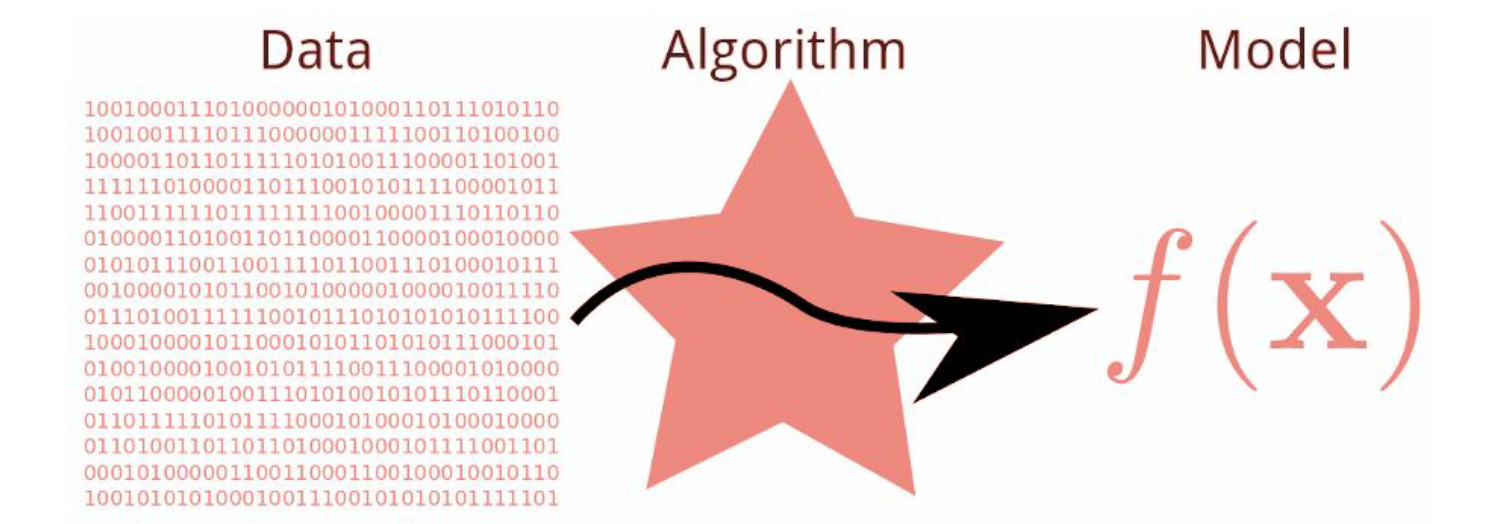
\includegraphics[scale=0.25]{data_model}

The training data produces a model or predictor, whereas the testing data produce a prediction. 
\section{Data}
Data can be a list of movies from IMDB which is easily representable. Although we need to use \textbf{features} when taking into consideration other examples. Features is how an algorithm view data and is generally represented with vectors. 

For example, classifying different apples, features could be the shape and colour of them.

The general problem with data for classification for example is that not all data is the same. For instance a banana can either be green or yellow. Although this is true we cannot go to deep with this so we use a probabilistic model called \textbf{data generating distribution}. Both training and test data are based on this. 

So in our previous example, we will generalize and say that bananas are yellow. 

\begin{definition}[Probability distribution]
	Describes how likely certain events are.
\end{definition}

High probability: round apples

Low probability: square apples

\section{Types of Learning}
\textbf{SUPERVISED LEARNING}\\
Supervised learning is when the algorithm is given labeled examples and the predictor should output a label. A further example of this is \textbf{classification}, where the model classifies from a pool of categories. 

Given a training set $T = {(x_i, y_i)}$ learn a function that predicts $y$ given $x$. x is multi-dimensional.

Some real world examples can be facial recognition, spam detection and character recognition. 

\textbf{Regression} is similar to classification only with real values (i.e. numbers).

\textbf{Ranking} the label is a ranking (most similar, most popular web pages etc.)


\textbf{UNSUPERVISED LEARNING}
The given data is without labels. 
Some examples are: 

\textbf{Clustering}, where the output is the general structure of the data set (clusters of data). Real world examples are image segmentation, social network analysis 

\textbf{Anomaly detection}

\textbf{Dimensionality reduction} 

\textbf{REINFORCEMENT LEARNING}

The idea is that the agent interacts with the environment and receives rewards based on behavior. 

\section{ML Ingredients}

\textbf{TASK}

A task represents the type of prediction being made to solve a problem. 

Assigning each input $ x \in \mathscr{X}$ to an output $y \in \mathscr{Y}$

\textbf{Data}

Data is basically the information required to solve a specific problem and as said previously is usually sampled from an unknown data generating distribution :

$\textbf{p}_{data}$ 

For classification and regression $\textbf{p}_{data} \in \triangle (\mathscr{X} \times \mathscr{Y})$

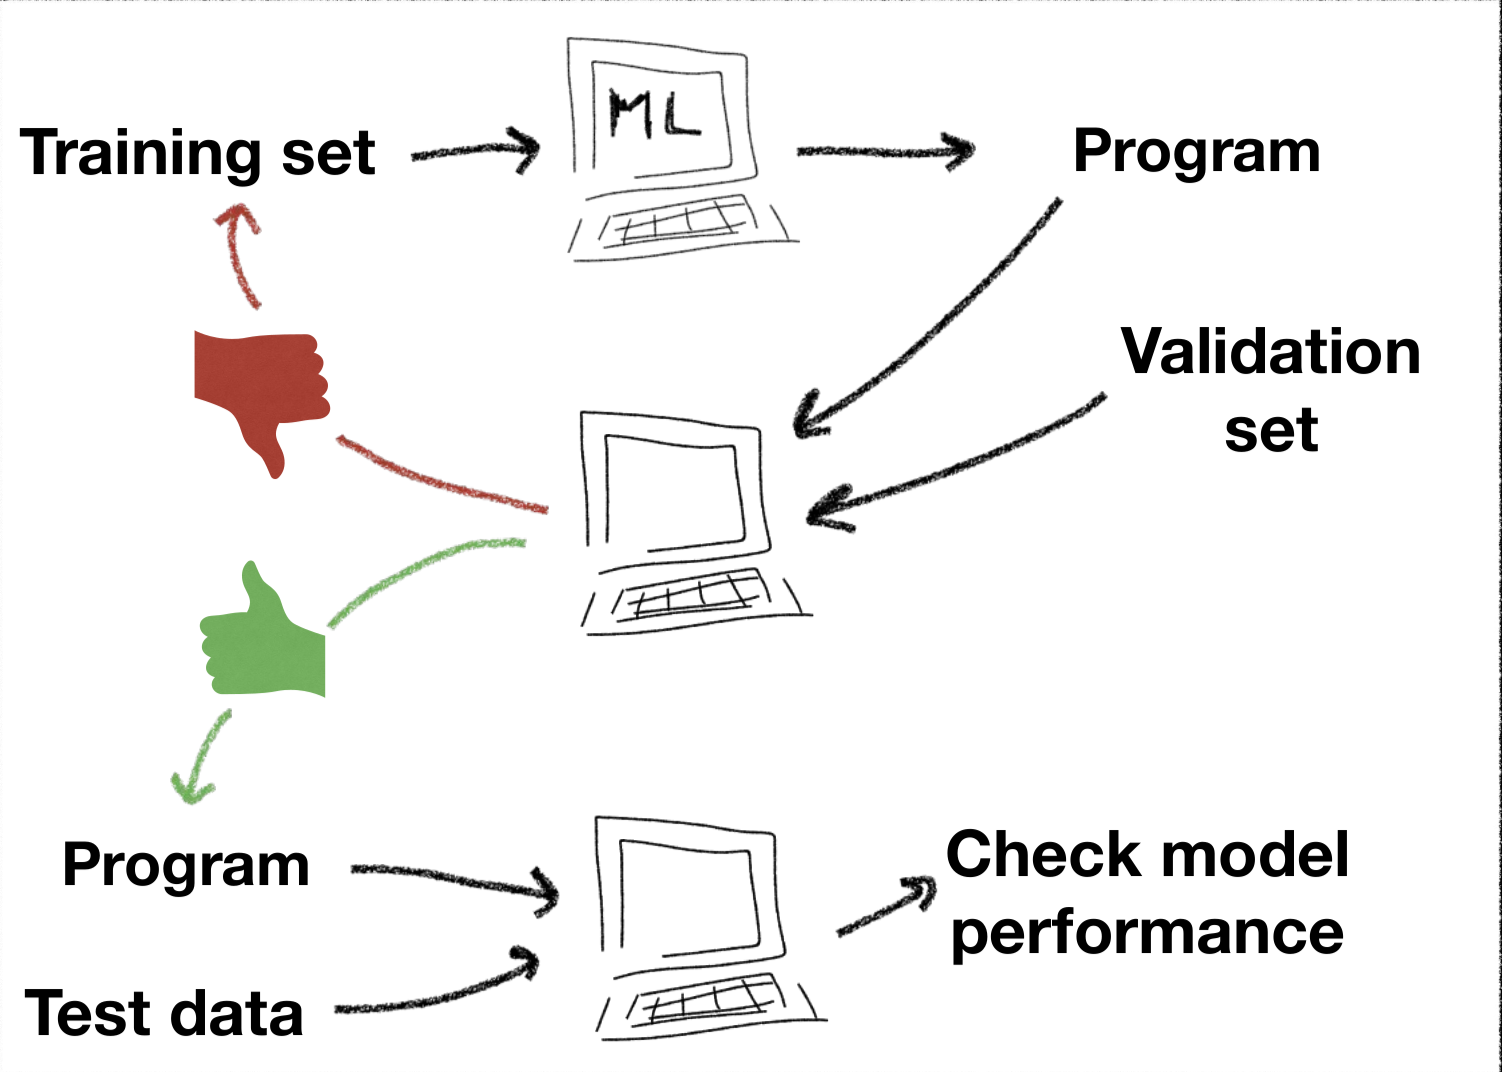
\includegraphics[scale=0.25]{datasets}

\textbf{Model and hypothesis space}

A model is like a program that solves the problem. There are various models (decision trees, neural networks.. ) and a set of them makes up the hypothesis space. 

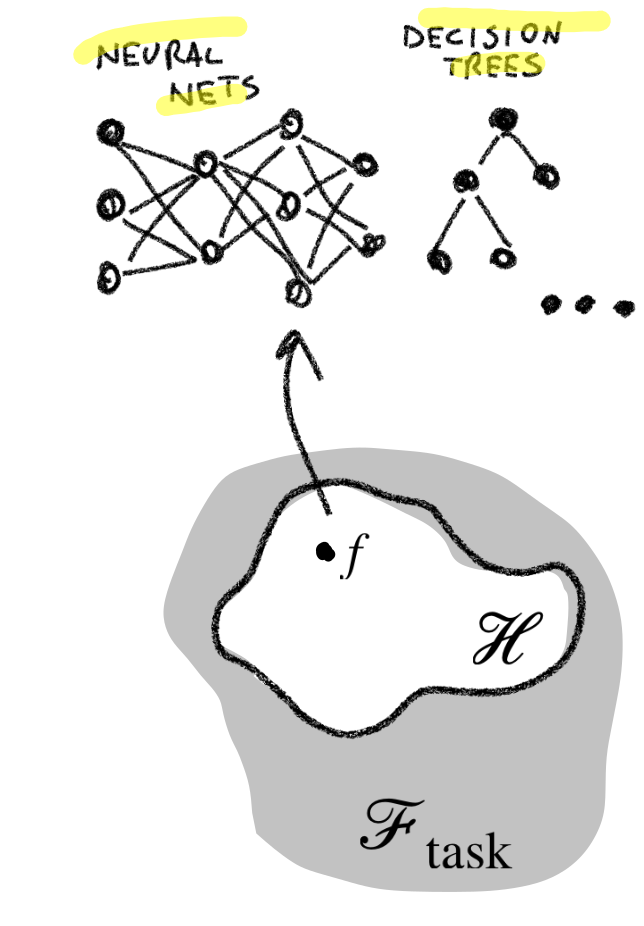
\includegraphics[scale=0.24]{hypothesis_space}

\textbf{The objective}

The objective is to minimize an error function $E(f,\textbf{p}_{data})$ to find the optimal function 

$f^{\star} =$ arg min $E(f,\textbf{p}_{data}) $.

This however is really hard to do because of the too large search space. 

The \emph{feasible target} is the optimal one in a restricted hypothesis space $\mathscr{H}$

$f^{\star}_{\mathscr{H}} =$ arg min $E(f,\textbf{p}_{data}) $.

This is also not doable because we do not have access to $\textbf{p}_{data}$
\\
The \emph{actual target} is then the following: 
\\

$f^{\star}_{\mathscr{H}} (\mathscr{D}_n) =$ arg min $E(f, \mathscr{D}_n) $. where $\mathscr{D}_n$ is a training set. 

The error function is usually specified as a pointwise-loss $\mathscr{l}(f,z)$ measuring the error of f on the training set z. 

The learning algorithm solves the optimization problem which targets the actual target. 


\chapter{K-Nearest Neighbor}

Imagine assigning each feature a numeric value, and putting them as coordinates in a feature space. To find which label to give to an example $d$ we can see the k-nearest neighbors. The correct label will be the one that has the majority in k neighbors. 


In cases where features are comparable (each feature has the same units) we will use the simple method of Euclidean Distance: 

\[
D(a,b) = \sqrt{(a_1-b_1)^2+(a_n-b_n)^2}
\]

\section{Decision boundaries}

\begin{definition}[Decision boundaries]
	Decision boundaries are places where the the classification of an example changes.
\end{definition}

These boundaries are a subset of the Voronoi diagram which divides the initial points distribution by equidistant lines. 

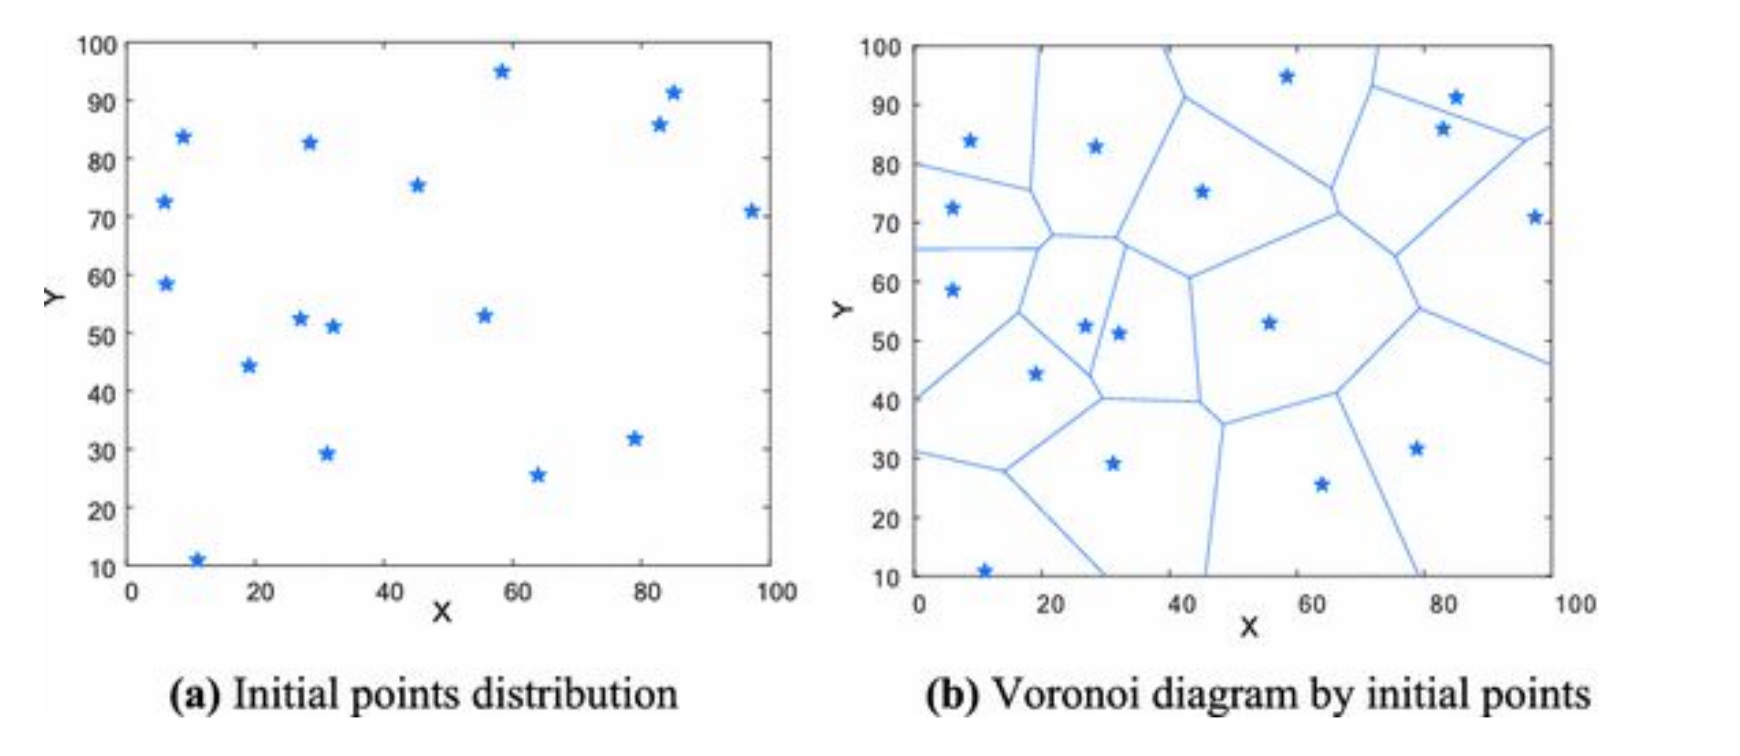
\includegraphics[scale=0.2]{voronoi}

Choosing K will have an effect on underfitting and overfitting.

\begin{definition}[Underfitting]
	Underfitting occurs when the model is not able to achieve a low error value on the training set
\end{definition}

\begin{definition}[Overfitting]
	Overfitting occurs when the gap between training set error and test set error is large
\end{definition}

Some heuristics come into play. It's important to choose an odd number to avoid ties. A general rule of thumb is that k should be lower than the square root of N training examples.
\\
\textbf{Weighted k-nn}, uses the same mechanics only that the examples are weighted which means that they will weigh in more in a vote situation.

\textbf{Lazy learning} is when an algorithm simply stores data and operates when given a test example.

\textbf{Eager learning} on the other hand is when given a training set, the algorithm constructs a classification model which then reutilizes. 

\section{Summary}
When is it useful:
\begin{itemize}
	\item Few features per instance
	\item Lots of training data
\end{itemize}

Advantages:

\begin{itemize}
	\item Training is very fast (lazy)
	\item Learn complex functions
\end{itemize}

Disadvantages:

\begin{itemize}
	\item Slow at query time
\end{itemize}





The main issue has to do with dimensionality. Every algorithm requires a dense data set, although K-NN requires to have at least one neighbor in each dimension, which makes for a very heavy computational load.

\chapter{Linear Models}
\section{Model assumptions}
Assumptions (when correct) are a great tool to improve an algorithm. They can however lead to overfitting. For K-NN the only assumption that's made is the fact that proximity relates to label. 

\begin{definition}[Bias]
	The bias of a model is how strong its assumptions are.
\end{definition}

K-NN and Decision Trees are considered to be low bias. 

\section{Linear models}
A high-bias assumption is linear separability, which means that the classes can be simply divided by a line (or hyperplane in n dimensions).

A line is defined by a pair of values: 

\[
0 = w_1f_1 + w_2f_2
\]

To classify we can input the values into the equation. If it's positive it will be above the line and viceversa.

In n-dimensions: 

\[
0 = b+ \sum_{i=1}^{n} w_if_i
\]

\section{Online learning}

This linear model is different because it sees one example at a time. This is useful when taking in data streams (for example from online resources).

The algorithm receives an unlabeled example, it predicts and if it is not correct it updates its model.

\section{Perceptron algorithm}
This is a linear model that constantly updates when not correct.

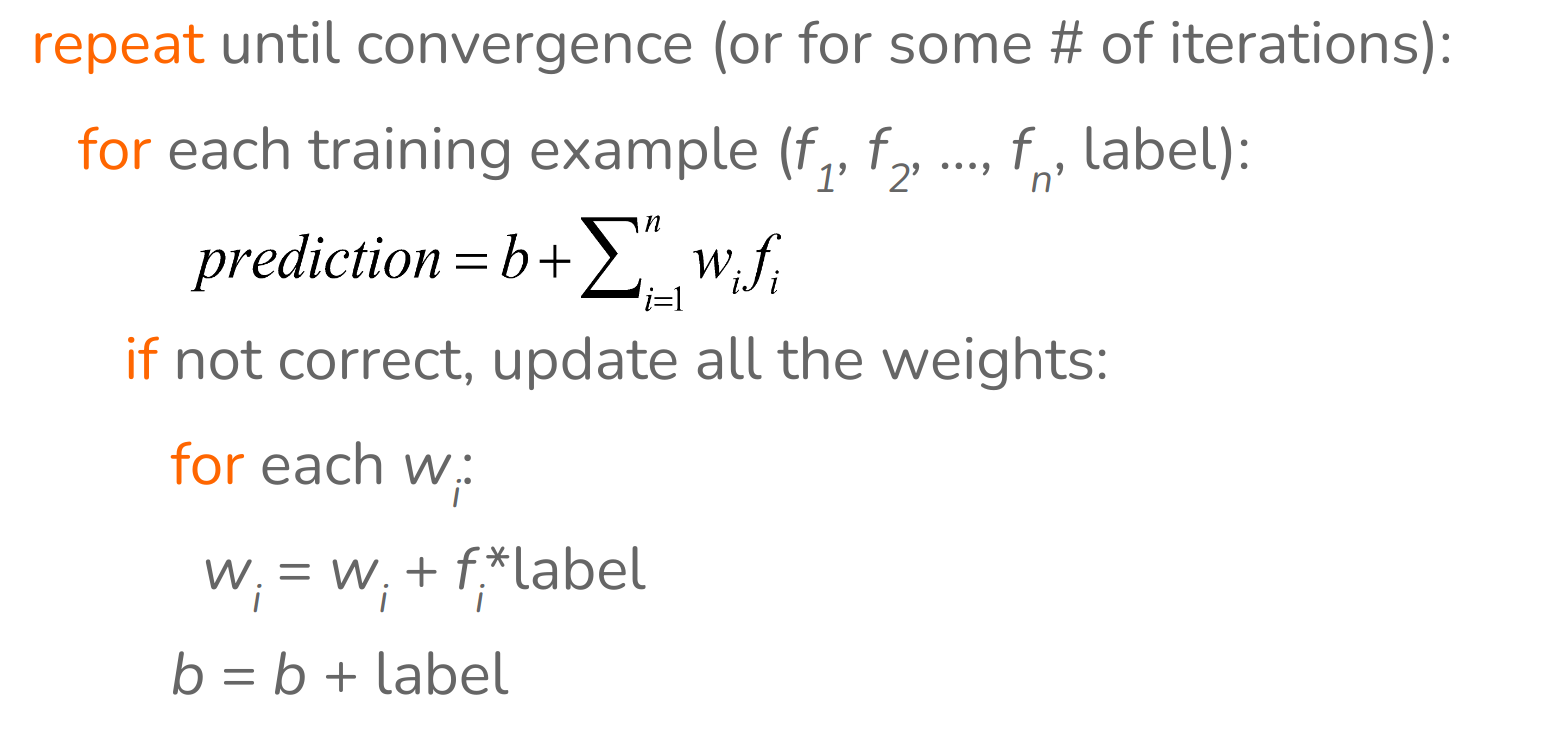
\includegraphics[scale=0.25]{perceptron}
\chapter{Multiclass Classification}
\begin{definition}[Binary classification]
	Given an input $\mathscr{X}$, an unknown distribution $D$ over $\mathscr{X}\times \{-1,1\}$
	a training set D compute a function f.
\end{definition}

\begin{definition}[Multiclass classification]
	Given an input $\mathscr{X}$ and a number K of classes, an unknown distribution $D$ over $\mathscr{X}\times K$
	a training set D compute a function f.
\end{definition}

None of the current methods work.

The main idea is to modify the perceptron by adding multiple lines. There are two approaches to this.

\section{One vs All (OVA)}

For each label L define a binary problem. All examples with L are positive, the rest is negative.

This poses a problem related to some areas in which it can either be two classes or none at all.

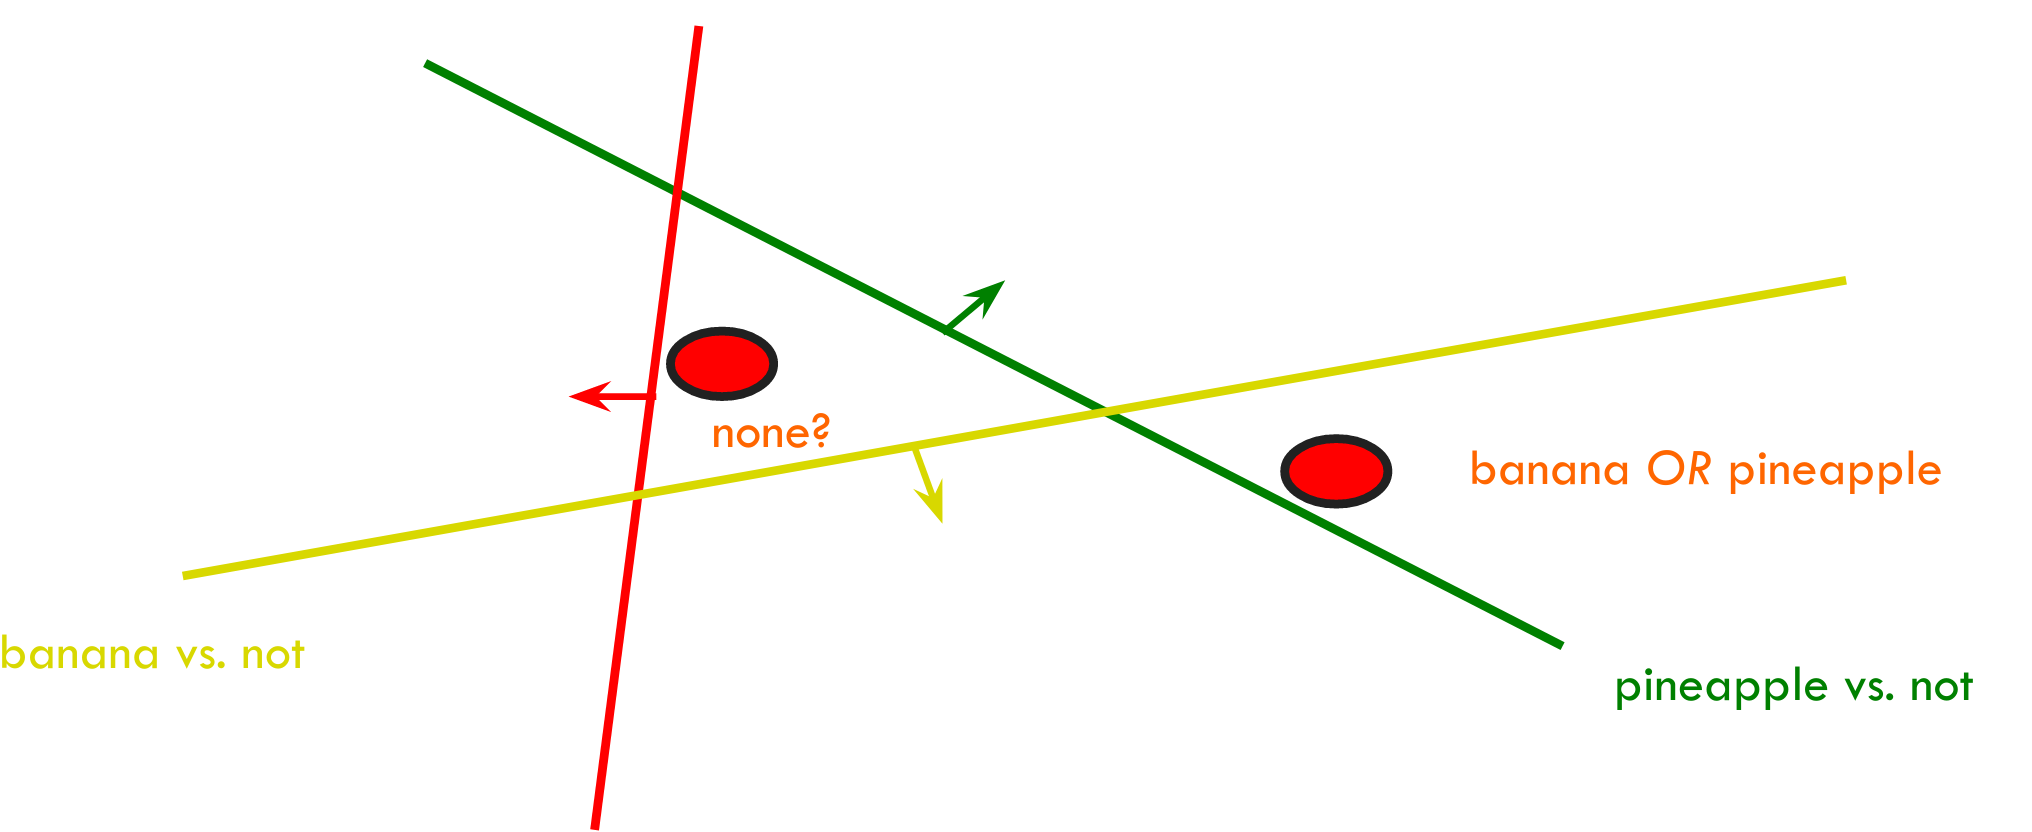
\includegraphics[scale=0.1]{multiclass}
 How to classify? 

Generally speaking the classifier should provide a level of confidence. To calculate this value we need to use decision boundaries and its distance from the hyperplane.
 
\section{All vs All (AVA)}
The idea behind AVA is to pair up each permutation of 1v1 pairs. Then, the classifier will receives all examples of i as a +1 and -1 for the j class. When a test point arrives we evaluate on all the $F_{ij}$ classifiers. 

\section{Summary}
AVA has faster training time but a slower test time. AVA has more chances of error at test time.

\textbf{Evaluation} comes when we need to evaluate a specific performance of an algorithm. Can be done through microaveraging, average over the examples, or macroaveraging, average of the average of each label.

\chapter{Gradient Descent}
\section{Model based machine learning}
There are 3 steps to this model:
\begin{enumerate}
	\item Pick a model (DT, perceptron)
	\item Pick a criterion to optimize
	\item Develop a learning algorithm
\end{enumerate}

In linear model: 
\begin{enumerate}
	\item 0 = b+ $\sum_{j=1}^{n} w_jf_j$
	\item $\sum_{i=1}^{n}1[y_y(w\cdot x_i + b) \leq 0]$ (0/1 Loss function aka the total number of mistakes)
	\item $argmin_{w,b}$ $\sum_{i=1}^{n}1[y_y(w\cdot x_i + b) \leq 0]$
\end{enumerate}

\section{Surrogate loss functions}
Minimizing the 0/1 Loss function is an NP-hard problem, because of the many local minima and any change in w can change drastically the result. Ideally we would want a convex function so to have at least one minimum.

By \textbf{surrogate loss function} we mean a loss function that provides an upper bound to the 0/1 loss function. 

\begin{itemize}
	\item 0/1 loss : $l(y,y') = 1[yy'\leq 0]$
	\item Hinge loss: $l(y,y') = max(0,1-yy')$
	\item Exponential loss: $l(y,y') = exp(yy')$
	\item Squared loss: $l(y,y') = (y-y')^2$
\end{itemize}

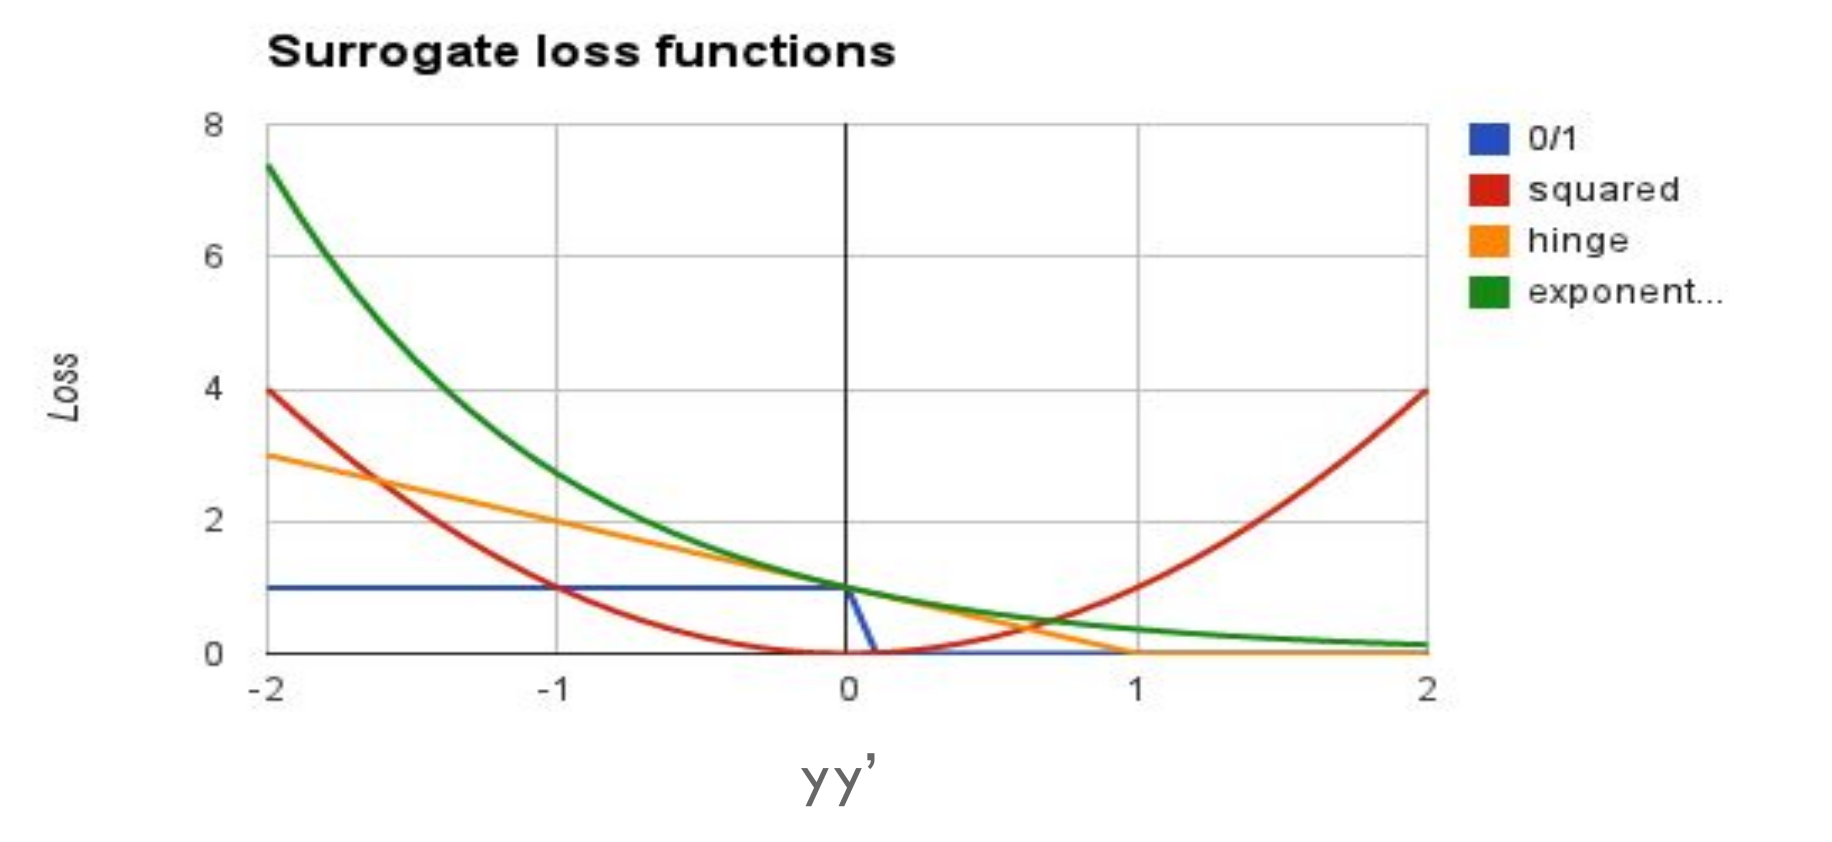
\includegraphics[scale=0.2]{surrogate}

\section{Gradient descent}
We use gradient descent to find a minimum in the function. 

The general approach is to choose a starting point $w$, calculate the derivative and move in that direction.

\[
w_j = w_j - \eta \frac{d}{dw_i}loss(w)
\]



$\eta$ is the rate at which we move and will change over time.

Since it's changing over time it can be implemented through a perceptron algorithm.

The main problem with gradient descent is local minima: 

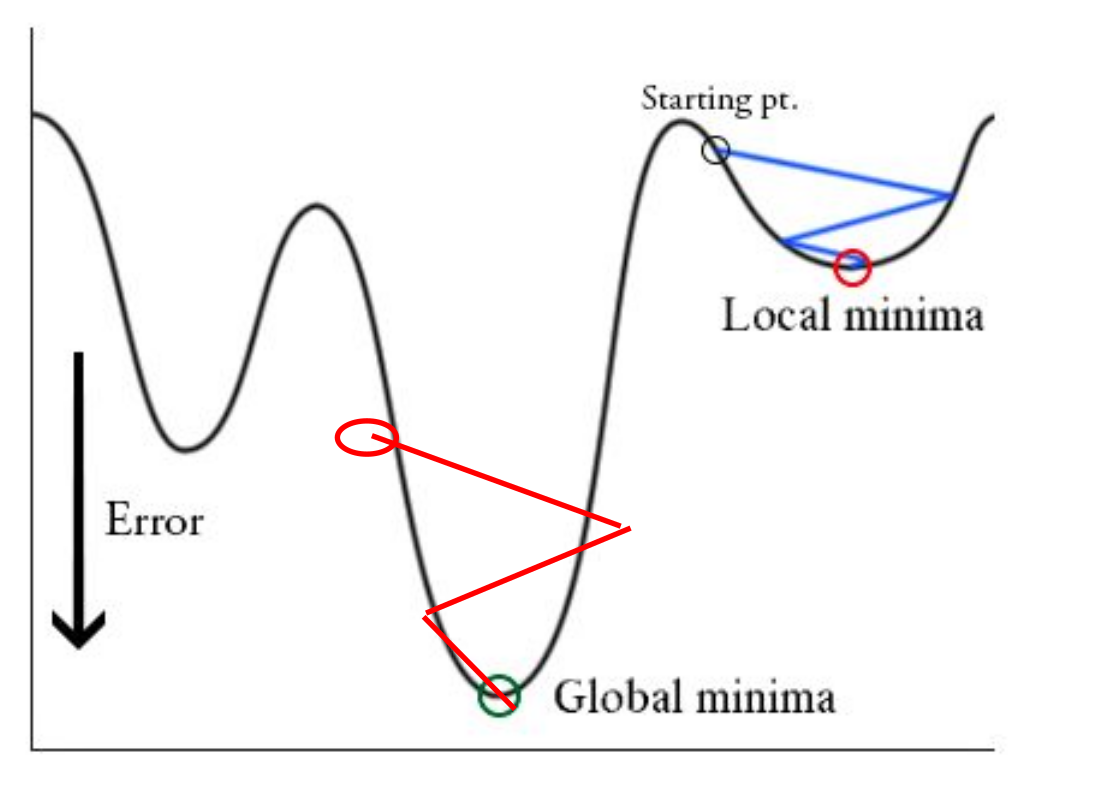
\includegraphics[scale=0.2]{local_minima}

\chapter{Regularization}
The problem with gradient descent remains the fact that since we're using it on the training set it can lead to overfitting. A solution to this is to use a regulalrizer.

\begin{definition}[Regularizer]
	An additional criterion to the loss function to avoid overfitting.
\end{definition}

More generally it regularizes the way we handle certain weights.

Generally, we do not want huge weights: if weights are large, a small change in a feature can result in a large change in the prediction.

Two common regularizers are: 

\begin{itemize}
	\item Sum of the weights: $\sum |w_j|$
	\item Sum of the squared weights: $\sqrt{\sum |w_j|^2}$
\end{itemize}

Sum of weights penalizes small values whereas square sum penalizes large values. 

P-norm: $\sqrt[p]{\sum |w_j|^p}$
\end{document}